% !TEX encoding = UTF-8 Unicode
% -*- coding: UTF-8; -*-
% vim: set fenc=utf-8
%\inputencoding{utf8}

\section{Autorizace}\label{sec:autorizace}

Protože v navrženém prototypu aplikace nejsou rozlišovány žádné pokročilejší uživatelské role, naprosto dostačuje jednoduchá kontrola přihlášení uživatele u jednotlivých přístupových bodů.
Tuto kontrolu provádí Middleware soubory, které validují každý příchozí požadavek od klienta.
Pokud se uživatel pokouší přistoupit ke koncovému bodu, který vyžaduje přihlášeného (resp\. nepřihlášeného) uživatele, Middleware soubory zkontrolují zda-li je uživatel přihlášen (resp\. odhlášen) a pak teprve serverová část aplikace pokračuje se zpracováním požadavku.

Složitější situace nastává v omezení přístupu uživatelů k jednotlivým dokumentům.
Uživatel může být k dokumentu přizván a jeho práva, tak nemusí odpovídat globálnímu nastavení práv pro sdílení dokumentu (sdílení pomocí veřejného odkazu).
Z tohoto důvodu jsem implementoval statickou třídu \texttt{DocumentVoter} (viz třídní diagram na obrázku~\ref{fig:DocumentVoter}).
Metody této třídy přijímají objekt uživatele (nebo hodnotu \texttt{null}, pokud uživatel není přihlášený) a objekt dokumentu, pro který chceme zjistit uživatelovo oprávnění.
Například metoda \texttt{DocumentVoter.can()} vrací Promise, která skončí úspěchem pouze v případě, kdy má předaný uživatel dostatečné oprávnění k provedení zvolené akce nad předaným dokumentem.

\begin{figure}[ht!]
    \centering
    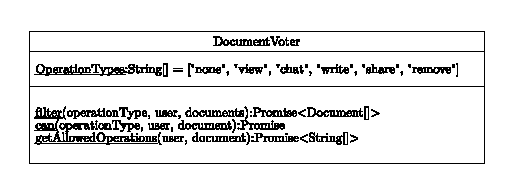
\includegraphics[width=\textwidth]{partials/realizace/DocumentVoter.pdf}
    \caption{Třídní diagram třídy DocumentVoter}\label{fig:DocumentVoter}
\end{figure}

Složitým problémem autorizace je omezení přístupu k samotnému editoru dokumentů a to nejen v případě, kdy uživatel nemá k dokumentu oprávnění, ale i v případě, že dokument vůbec neexistuje.
Klientská část aplikace nemá přístup k DB a nemůže tedy zjistit, zda-li se má editor vůbec aktuálnímu uživateli zobrazit, či která část má zůstat skryta, protože k ní uživatel nemá dostatečné oprávnění.
Proto klientská část pro každý dokument zahájí spojení se serverem, který po přijetí zprávy Připojení k dokumentu (viz sekce~\ref{sec:komunikaceVeSkutečnémČase} o komunikaci) rozhodne zda-li uživatele připojí (a vrátí seznam operací, ke kterým má uživatel dostatečné oprávnění) nebo odešle zprávu Chyba a spojení ukončí.

Z tohoto důvodu se může stát, že aplikace před zobrazení chyby o nenalezení dokumentu na zlomek vteřiny zobrazí editor dokumentu.
Editor je v uzamčeném stavu a neumožňuje uživateli editaci, ani žádnou jinou operaci nad dokumentem, ale jeho zobrazení je nutné pro správné vytvoření instance textového editoru.
